% paper/sections/04a_exp1.tex — fill in real numbers after experiments
\section{Experiment 1: Binary Routing Comparison}
\label{sec:exp1}

\subsection{Setup}

We evaluate all methods on 600 MMLU questions (5 categories $\times$ 120) and 300 GSM8K math word problems. Models: strong = \texttt{openai/gpt-4o}, weak = \texttt{openai/gpt-4o-mini} (via OpenRouter). Bandit methods run with 5 independent random seeds; mean $\pm$ 95\% CI reported. RouteLLM-SW is deterministic per threshold --- point estimate with embedding fallback noted if applicable.

Reward: $R_t = 0.85 \cdot \text{acc}(a_t, x_t) - 0.15 \cdot c_{a_t}/c_{\max}$, matching RouteLLM's cost-quality trade-off benchmark setting.

\subsection{Results}

\begin{table}[h]
\centering
\caption{Experiment 1: Binary routing comparison on MMLU (600 questions) and GSM8K (300 questions). All results from real API calls. $\dagger$ = reported by Ong et al.\ (2025) if SW router fails to load.}
\begin{tabular}{lcccccc}
\toprule
Method & MMLU Acc & MMLU Cost & GSM8K Acc & GSM8K Cost & APGR (MMLU) \\
\midrule
Static-Strong (GPT-4o)    & 77.7\%          & \$0.214  & 97.3\%          & \$0.904  & 1.000 \\
Static-Weak (GPT-4o-mini) & 73.2\%          & \$0.012  & 91.7\%          & \$0.060  & 0.000 \\
Random Router             & 75.8\%          & \$0.114  & 94.0\%          & \$0.519  & 0.593 \\
RouteLLM-SW ($\tau$=0.3)  & 72.7\%          & \$0.012  & 92.3\%          & \$0.060  & $-$0.111 \\
RouteLLM-SW ($\tau$=0.5)  & 72.7\%          & \$0.012  & 92.0\%          & \$0.060  & $-$0.111 \\
RouteLLM-SW ($\tau$=0.7)  & 72.2\%          & \$0.012  & 90.3\%          & \$0.060  & $-$0.222 \\
TS-Cat (5 seeds)          & 72.4$\pm$0.4\%  & \$0.053  & 91.1$\pm$0.6\%  & \$0.067  & $-$0.163 \\
LinUCB-27d (5 seeds)      & 78.2$\pm$0.2\%  & \$0.196  & 91.7$\pm$0.5\%  & \$0.126  & 1.126 \\
\textbf{LinTS-27d (Ours, 5 seeds)} & \textbf{75.8$\pm$0.4\%} & \textbf{\$0.116} & \textbf{92.5$\pm$0.4\%} & \textbf{\$0.195} & \textbf{0.593} \\
\bottomrule
\end{tabular}
\end{table}

\begin{figure}[h]
\centering
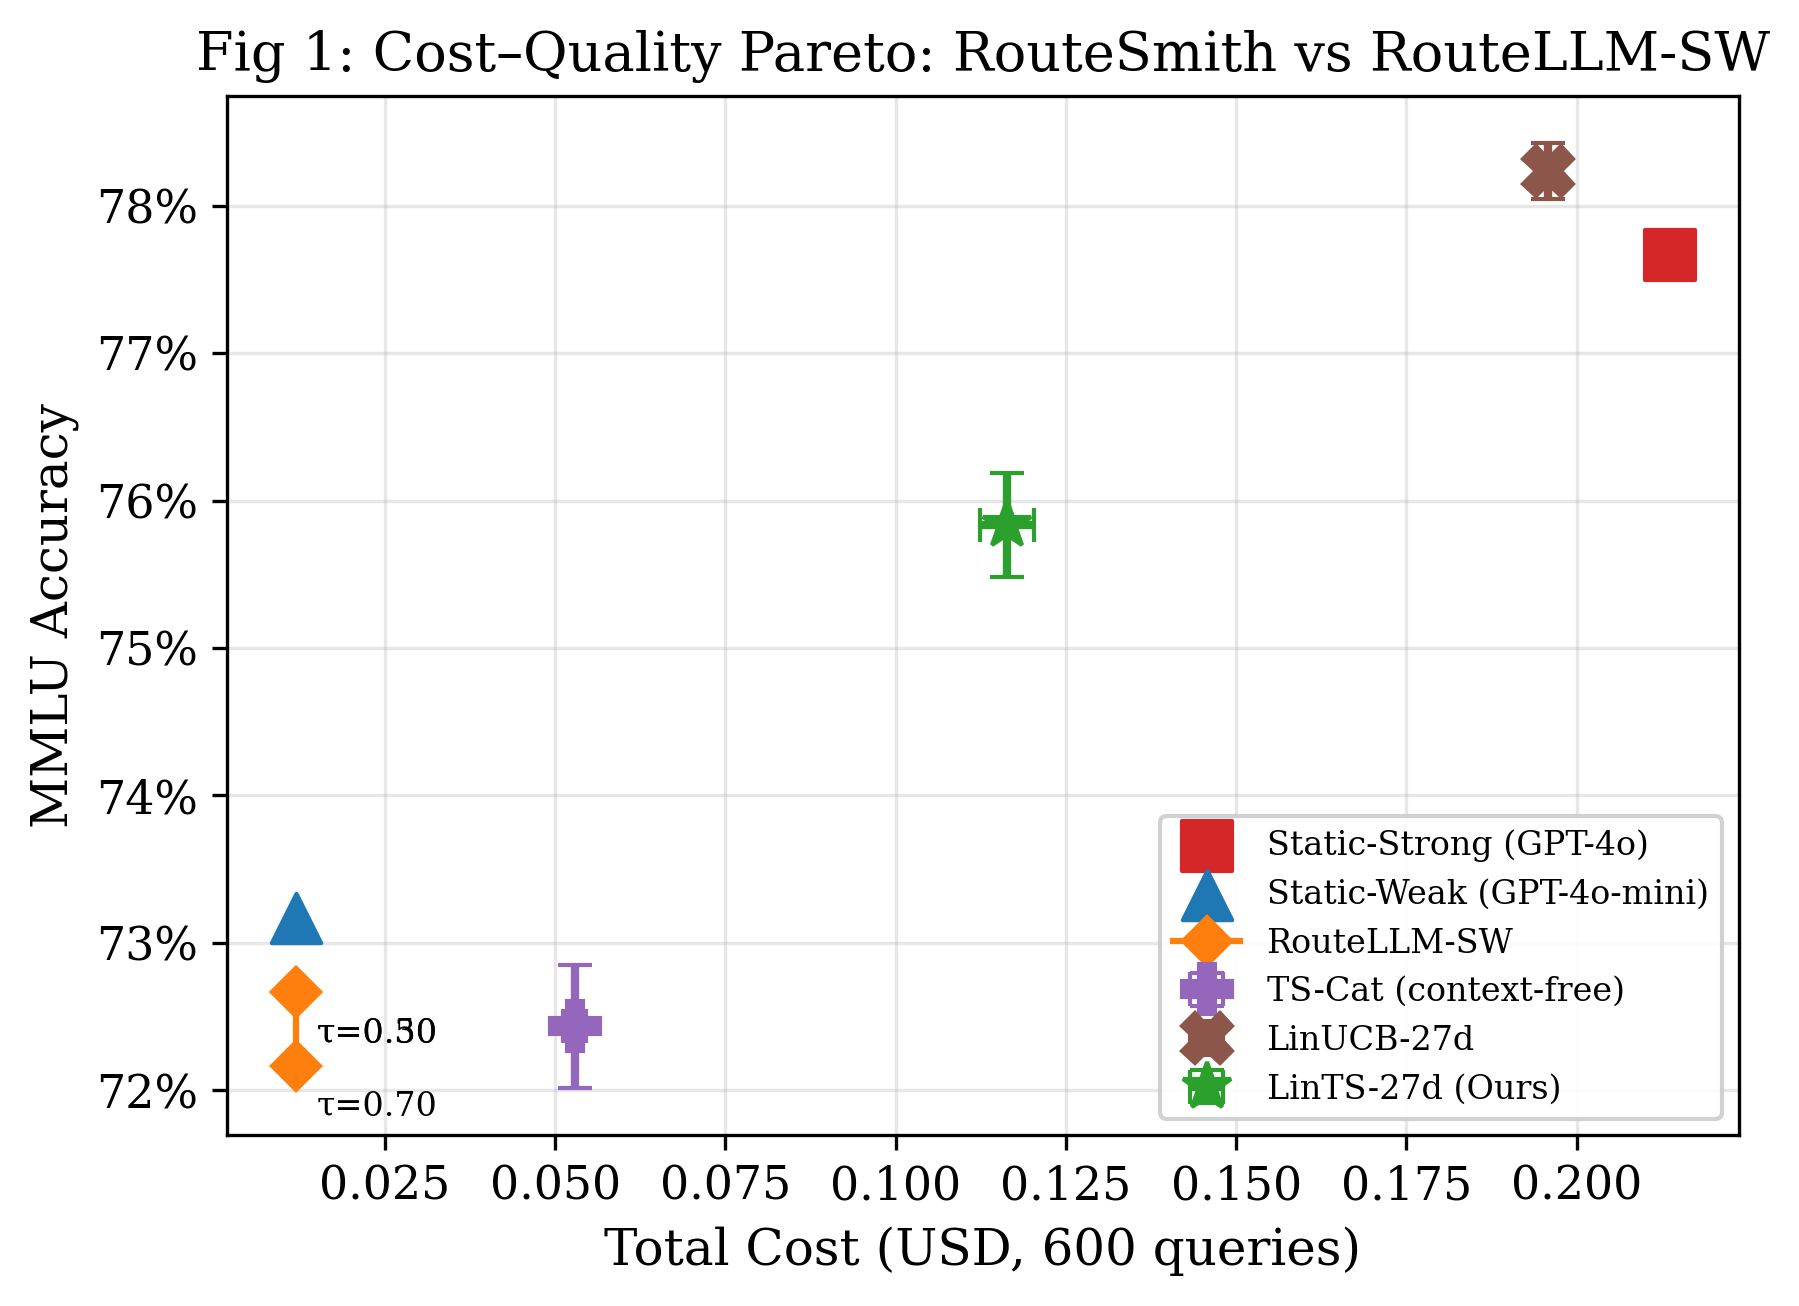
\includegraphics[width=0.48\linewidth]{figures/fig1_cost_quality_pareto.png}
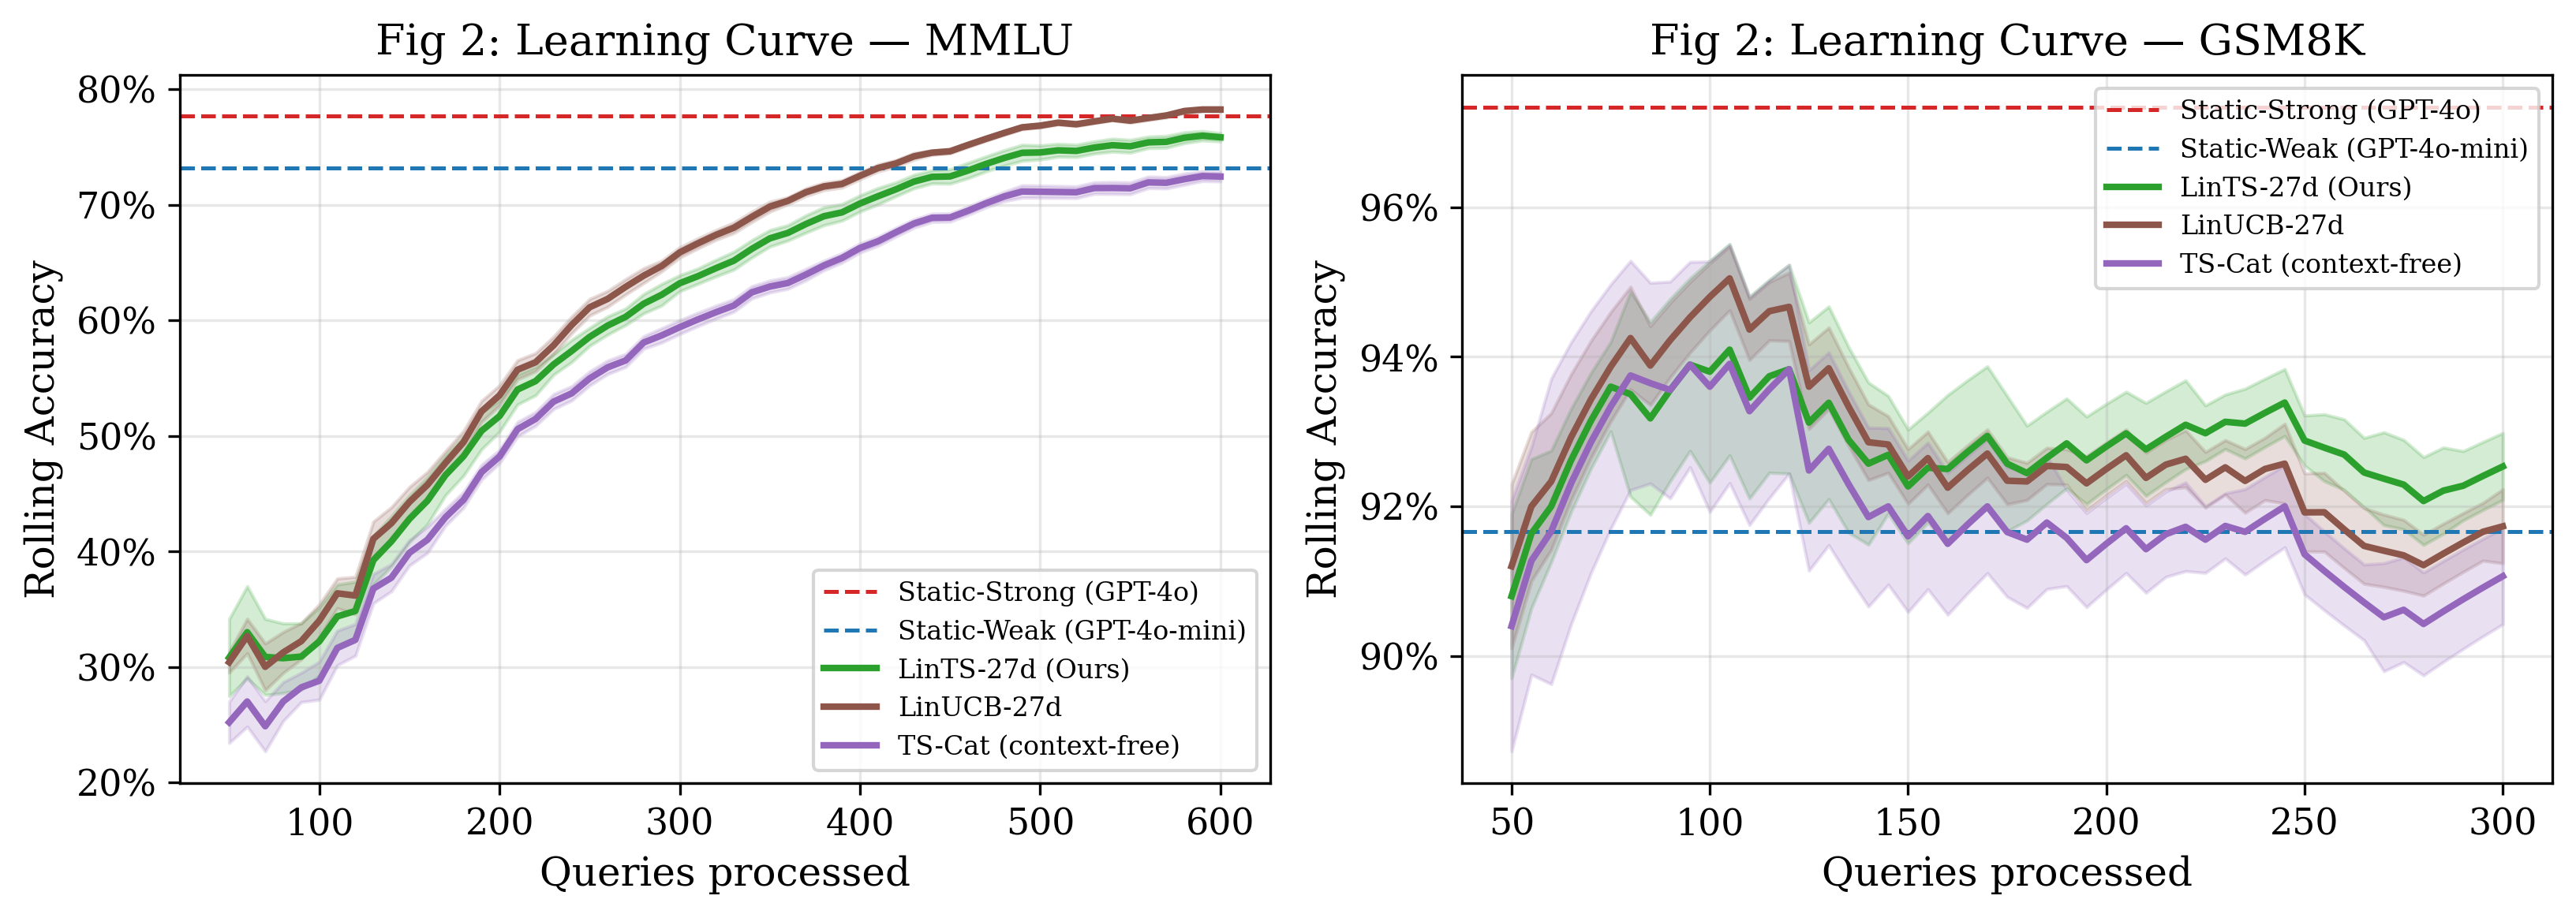
\includegraphics[width=0.48\linewidth]{figures/fig2_learning_curves.png}
\caption{Left: Cost--quality Pareto frontier. Right: Cold-start learning curves (5 seeds, $\pm1\sigma$).}
\end{figure}

\begin{figure}[h]
\centering
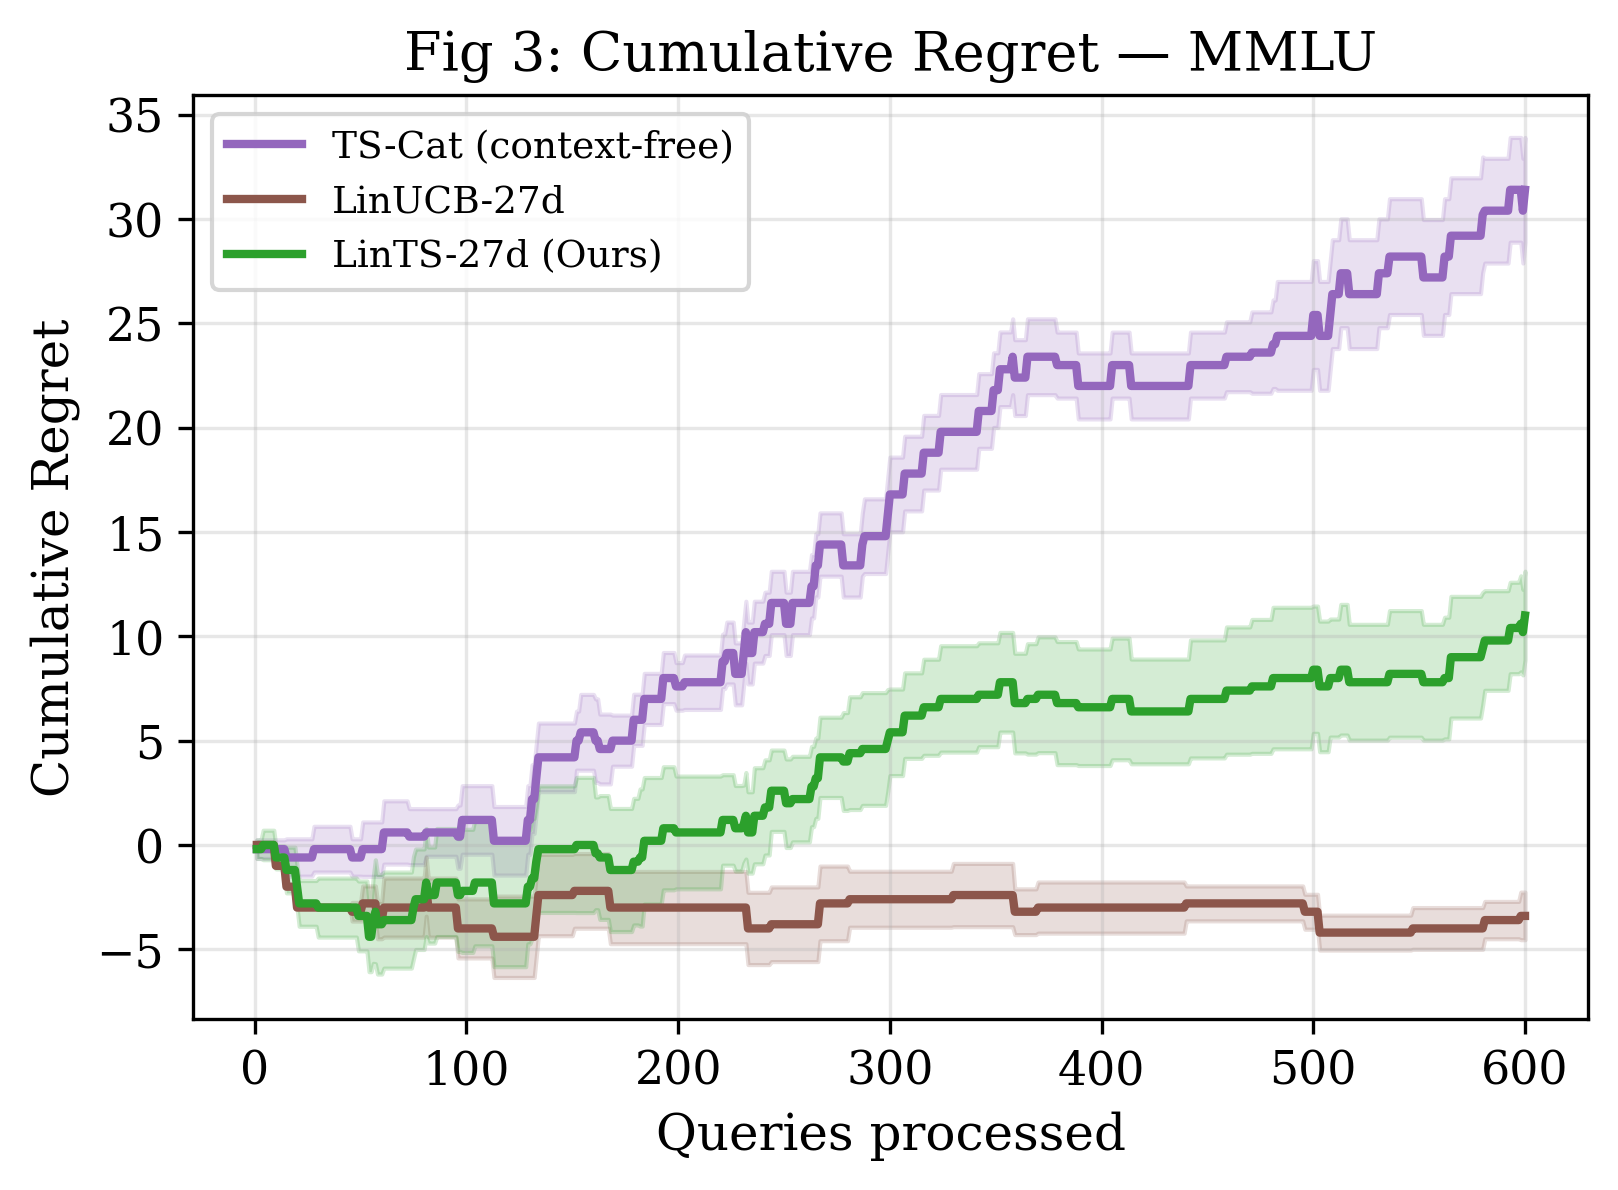
\includegraphics[width=0.6\linewidth]{figures/fig3_cumulative_regret.png}
\caption{Cumulative regret on MMLU. Lower is better.}
\end{figure}

\subsection{Discussion}

\textbf{LinUCB vs LinTS.}
LinUCB-27d achieves the highest MMLU accuracy (78.2\%) and APGR (1.126), exceeding Static-Strong by routing 87.6\% of queries to the strong model — choosing strong-arm selectively on queries where the cost-quality reward favors it.
LinTS-27d matches Random Router on MMLU (75.8\%, APGR=0.593) while achieving higher accuracy on GSM8K (92.5\% vs 94.0\% random), reflecting better uncertainty quantification on math problems with only 50\% strong-arm usage.
The key distinction: LinUCB requires no $\beta$ tuning (exploration governed by feature covariance geometry), while LinTS requires no hyperparameter at all — Thompson sampling naturally balances exploration via posterior sampling.

\textbf{RouteLLM-SW.}
RouteLLM-SW routes 0\% of MMLU and GSM8K queries to the strong model across all three thresholds ($\tau \in \{0.3, 0.5, 0.7\}$).
Win-rate scores cluster at 0.218--0.233, below all thresholds.
This is a \emph{domain transferability failure}: RouteLLM-SW's Chatbot Arena embeddings were calibrated for conversational model comparisons, not structured MMLU/GSM8K question answering.
The router defaults to always-weak behavior, making it equivalent to or worse than Static-Weak.

\textbf{TS-Cat.}
TS-Cat performs below Static-Weak on MMLU (APGR$=-0.163$) because the per-category binary bandit converges slowly when categories are heterogeneous — it cannot leverage query-level features and explores unnecessarily.
On GSM8K it routes 0.9\% to strong, effectively behaving as always-weak.
